\section{Implementation}
\begin{frame}{Overview}
    \begin{itemize}
        \item The implementation of the compiler is differentiate into four different stages:
        \begin{enumerate}
            \item the lexical and syntactic analysis,
            \item semantic analysis,
            \item code generation, and % at generation time
            \item optimizations
        \end{enumerate}
        \item The process is managed by a static compiler class.
        \item It parses the command line parameters, handles the input and output of files, and calls the different stages.
    \end{itemize}    
    \begin{figure}[htp]
        \centering     
        \lstinputlisting[style=bashstyle]{../figures/code/slides/cli_example.bash}
        \caption{A command line interface example.}
    \end{figure}
\end{frame}

\begin{frame}{Symbols and Symbol Table}
    \begin{minipage}{.45\textwidth}
        \begin{itemize}
            \item Through out the whole compilation process, the symbol table is used to save and propagate symbol information.
            \item Additionally, it handles higher level concepts such as variable contexts.
            \item It contains a dictionary that maps identifier to the symbol objects.
            \item All symbol objects are derived from an abstract symbol class.
        \end{itemize}    
    \end{minipage}
    \begin{minipage}{.50\textwidth}
        \centering
        \begin{figure}[htp]
            \centering
            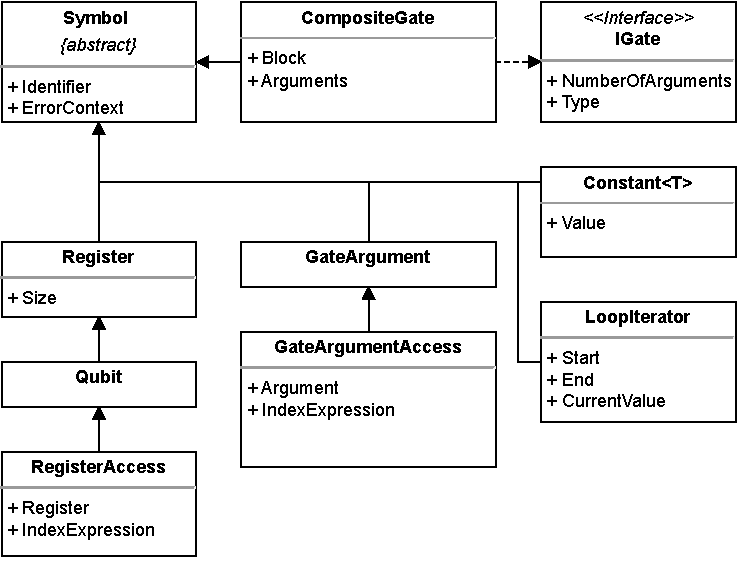
\includegraphics[]{../figures/drawio/slides/uml_symbols.pdf}
            \caption{A diagram showing the hierarchy of symbol classes.}
            % \label{fig:implementation_uml_errors}
        \end{figure}
    \end{minipage}
\end{frame}

\subsection{Lexical and Syntactic Analysis}
\begin{frame}{Lexical and Syntactic Analysis}
    \begin{itemize}
        \item The first compilation stage is the lexical and syntactic analysis.
        \item Both the lexer and parser are created with the ANTLR4 tool.
        \item It generates the source code based on a given grammar. 
        \item The implementation of the grammar is a more elaborate version of the syntax given previously.
    \end{itemize}
    \begin{figure}[h]
        \centering
        \lstinputlisting[style=ANTLR]{../figures/code/implementation/grammar_structure.g4}
        \caption{The basic structure of parsing rules for Luie.}
    \end{figure}
\end{frame}

\subsection{Semantic Analysis}
\begin{frame}{Semantic Analysis}
    \begin{itemize}
        \item The next step is the semantic analysis.
        \item An analysis without any context is not sufficient for non-syntactic constraints of the program.
        \item For example, the syntactic analysis may ensure gate declarations are always at the beginning of a program, but it cannot ensure that all identifiers in a gate application were previously defined.
        \item Our semantic analysis is divided into two parts:
        \begin{enumerate}
            \item the declaration analysis and
            \item the type checking.
        \end{enumerate}
        \item Both parts are implemented as ANTLR listener classes. 
        \item These traverse the parse tree and call both an enter and exit function for each grammar rule, \eg, \texttt{EnterBlock} and \texttt{ExitBlock}.
    \end{itemize}
\end{frame}

\subsection{Semantic Analysis}
\begin{frame}{Semantic Analysis}
    \begin{itemize}
        \item The declaration analysis ensure that all identifiers used were previously declared and all identifiers used in declarations are not already declared.
        \item This includes throwing warnings for declared but unused identifiers.
        \item Additionally, it prevents the use of a qubit in a code block that is guarded by the same qubit because this would lead to irreversible gates.
        \item The type checking ensures that symbols are used in the correct context.
        \item For example, while a qubit symbol can be used as the argument for a gate application, it does not represent a classical numerical value and, therefore, cannot be used in the context of a factor.
        \item Since we do not give the type of composite gate argument, its body cannot be type checked and any invalid types are thrown at generation time. 
    \end{itemize}
\end{frame}

\subsection{Code Generation}
\begin{frame}{Code Generation}
    \begin{itemize}
        \item First, the parse tree is traversed and the source code is translated to an in-memory representation.
        \item Next, this source code representation (SCR) is translated to the target code representation (TCR).
        \item Then, the TCR can be translated directly to the textual OpenQASM code.
        \item We want to go through the process with the example program from before.
        \item For simplicity, the named constant was replaced with a constant value.
    \end{itemize}
    \begin{figure}
        \centering
        \lstinputlisting[style=Luie, basicstyle=\large\ttfamily]{../figures/code/implementation/codeGen_example.luie}
        \caption{An example Luie program to show the code generation process.}
    \end{figure}
\end{frame}

\begin{frame}{Source Code Representation}
    \begin{minipage}{.45\textwidth}
        \begin{itemize}
            \item All SCR objects implement the translatable interface, which requires a translation function.
            \item The are three main translatables: the code block, statement, and declaration classes.
            \item The block contains a list of translatables and is used for both the main block and the body of some statements.
            \item The declaration consists only of register declarations; the compile-time-only declarations are only saved in the symbol table. 
        \end{itemize}    
    \end{minipage}
    \begin{minipage}{.50\textwidth}
        \centering
        \begin{figure}[htp]
            \centering
            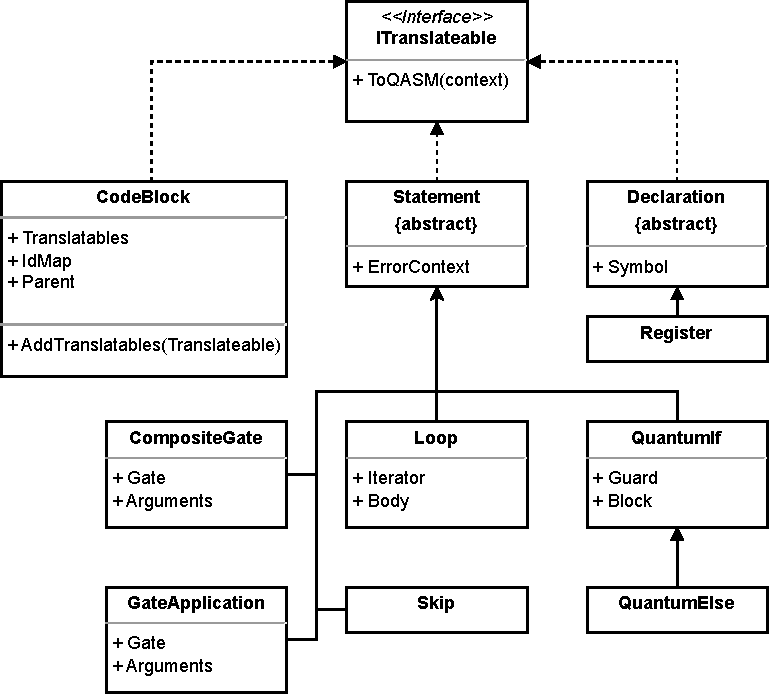
\includegraphics[]{../figures/drawio/slides/uml_translateables.pdf}
            \caption{A diagram showing the hierarchy of translatable classes.}
            % \label{fig:implementation_uml_errors}
        \end{figure}
    \end{minipage}
\end{frame}

\begin{frame}{Source Code Representation --- Example}
    \begin{minipage}{.60\textwidth}
        \begin{itemize}
            \item Any translation always consists of the main block.
            \item It contains three translatables.
            \item The first two are the declarations and the last is the composite gate statement.
            \item The gate's body contains only an if-statement, which, in turn, contains a loop statement.
            \item The loop statement consists of a gate application. 
        \end{itemize}   
        \vfill
        \begin{figure}
            \centering
            \lstinputlisting[style=Luie, basicstyle=\large\ttfamily]{../figures/code/slides/luie_example_reduced.luie}
            \caption{An example Luie program to show the code generation process.}
        \end{figure} 
    \end{minipage}
    \begin{minipage}{.35\textwidth}
        \centering
        \begin{figure}[htp]
            \centering
            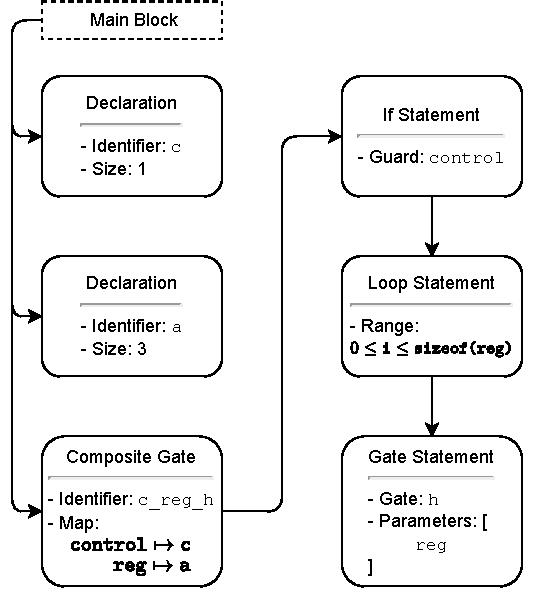
\includegraphics[]{../figures/drawio/codeGen_sourceCode_example.pdf}
            \caption{The SCR of the example program.}
            % \label{fig:implementation_uml_errors}
        \end{figure}
    \end{minipage}
\end{frame}

\begin{frame}{Target Code Representation}
    \begin{itemize}
        \item The basis of the TCR is the \texttt{QASMProgram} object.
        \item It contains a list of \texttt{Code} objects, which are either declarations of gate applications. 
        \item All SCR objects can be translated to a list of code objects and appended to the program object.
        \item The translations are as described in translation section.
        \item For example, a if-statement adds a control qubit to all gate applications in the block translation.
        \item All code objects implement a \texttt{ToCode} function that returns the textual representation of the statement.
        \item To translate the program object, the code objects are simply iterated, converted to text, and written to a file. 
    \end{itemize}
    \vfill
    \begin{align*}        
        ct(\texttt{qif } qArg \texttt{ do } blk \texttt{ end}, st) = \ &  control(qt(qArg, st), bt(blk, st)) \\
    \end{align*}
\end{frame}

\begin{frame}{Target Code Representation --- Example}    
    \begin{minipage}{.45\textwidth}
        \centering
        \begin{figure}[htp]
            \centering
            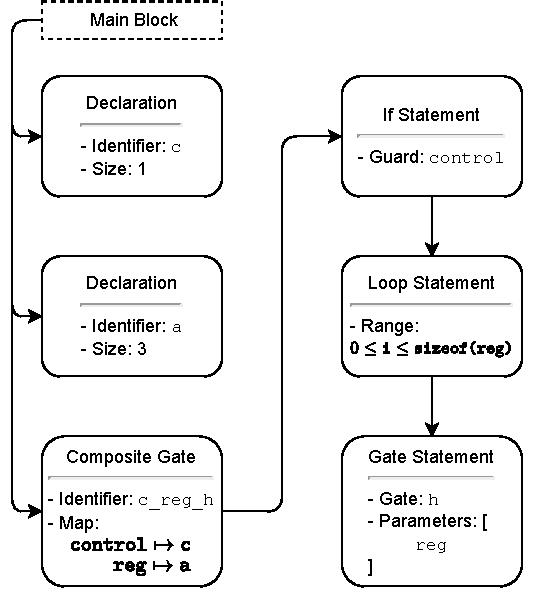
\includegraphics[]{../figures/drawio/codeGen_sourceCode_example.pdf}
            \caption{The SCR of the example program.}
            % \label{fig:implementation_uml_errors}
        \end{figure}
    \end{minipage}
    \hfill
    \begin{minipage}{.45\textwidth}
        \centering
        \begin{figure}[htp]
            \centering
            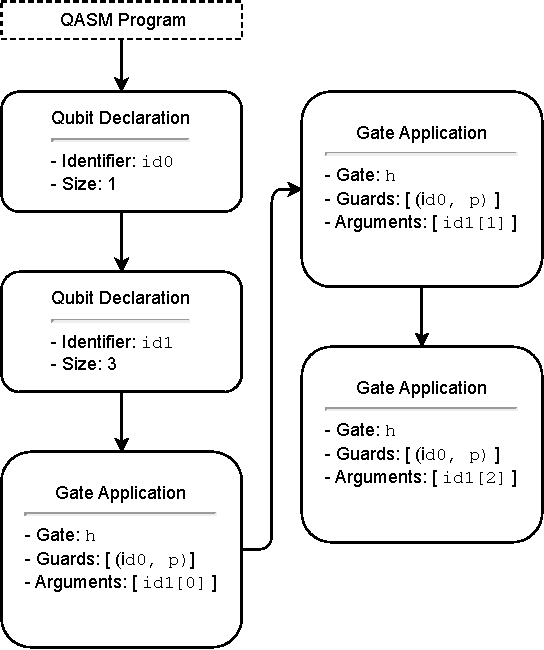
\includegraphics[]{../figures/drawio/codeGen_targetCode_example.pdf}
            \caption{The TCR of the example program.}
            % \label{fig:implementation_uml_errors}
        \end{figure}
    \end{minipage}
\end{frame}

\begin{frame}{Translated Example Program}    
    \begin{minipage}{.40\textwidth}
        \begin{itemize}
            \item ... 
            \item ... 
            \item ... 
            \item ... 
        \end{itemize}
    \end{minipage}
    \hfill
    \begin{minipage}{.55\textwidth}
        \centering
        \vfill
        \begin{figure}
            \centering
            \lstinputlisting[style=QASM,basicstyle=\Large\ttfamily]{../figures/code/implementation/codeGen_example.qasm}
            \caption{The OpenQASM translation of the example Luie program.}
            % \label{fig:codeGen_target_example}
        \end{figure}
        \vfill
    \end{minipage}
\end{frame}

\subsection{Optimization}
\begin{frame}{Optimization}
    \dots
\end{frame}
